\section{Improvements to Matrice 100 hovering performance through additional sensors and control (J.~Lim)}
\label{sec:hoveringcontrol}

The DJI Matrice 100 equipment had an attachable guidance system which has optic flow ultrasound sensors. This guidance system has the main central unit along with the frame surrounding it so that the four usable sensors can be adjusted in position for whichever direction you want to avoid colliding in. We worked on configuring the drone setup if it was to fly with the guidance system along and still have space to attach the extraction arm and end effect. The configuration was valid, however, there were some issues that arose after configuring the drone. The guidance system must be powered from the drone by using the XT60 power adapter cord, however, the length of the XT60 power cord was not long enough to reach the power outlet that connects to the drone and the power inlet for the guidance system. 

As seen in the pictures, one sensor was attached below the drone while the other three sensors were attached to the main frame of the guidance system up top. The reason for this configuration was because during the sample recovery mission, the drone needs to stay stable when hovering. The guidance system is able to detect velocity between \SIrange{0}{16}{\meter\per\second} and has an accuracy of \SI{0.04}{\meter\per\second} velocity detection (\SI{2}{\meter} above the ground). The sensors’ effective range is between \SIrange{0.20}{20}{\meter}. Because the effective range is up to \SI{65}{\foot}. The bottom sensor can track how the drone is moving based on what’s below the drone whether it is a sloped ground or the ocean next to the cliff. 

The guidance system can prove to be very helpful in the mission because stability of the drone during the sample recovery mission was one of the main issues the mission was difficult. If the drone is able to stabilize at an altitude high enough where there sensors are still effective, the drone may be stable enough where the drone pilot doesn’t have to worry about stabilizing the drone when hovering in close proximity of the plant. This also has the potential to change the way the extraction device is designed in which the extraction device might not need to be countering the drone’s movement while hovering, but rather just able to focus on grabbing the plant and securing the plant sample. 

\begin{figure}
\begin{center}
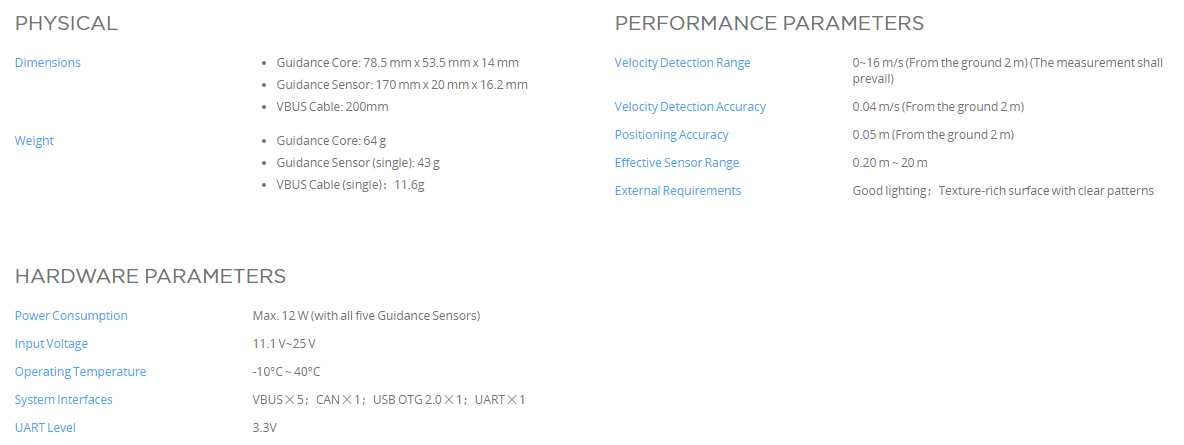
\includegraphics[width=\columnwidth]{figures/hovering1.png}
\end{center}
\caption{Specifications of the guidance system}
\label{fig:hovering1}
\end{figure}

\begin{figure}
\begin{center}
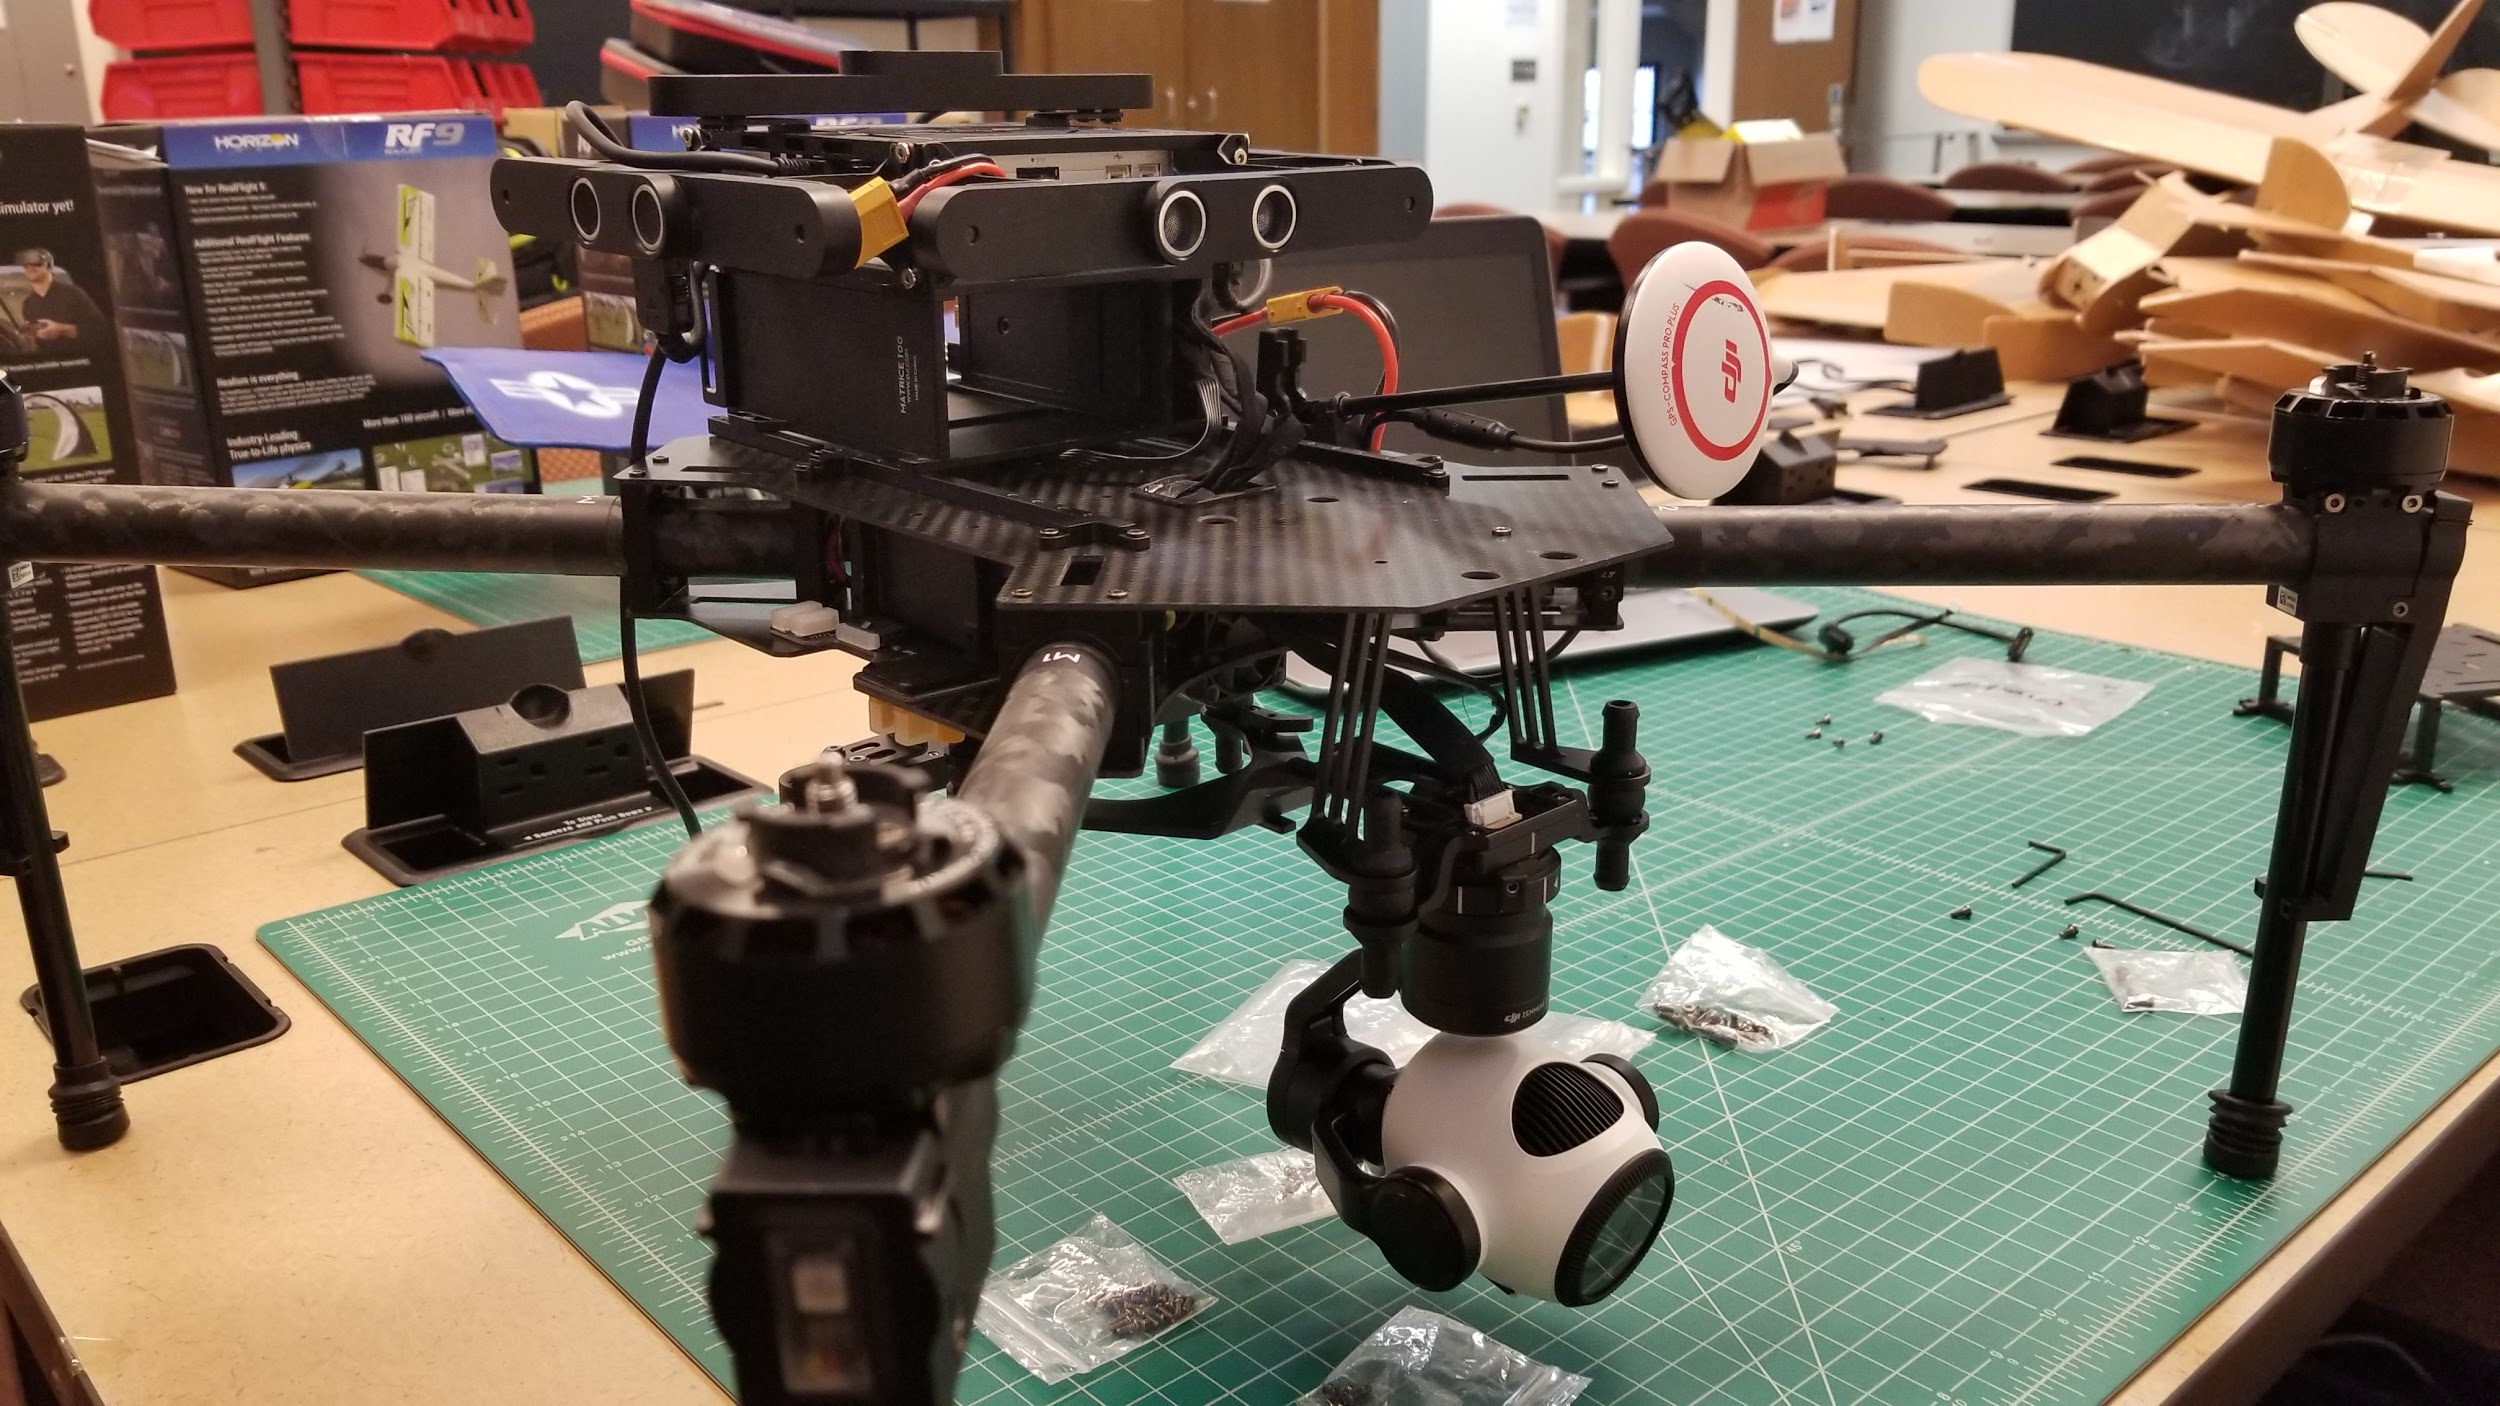
\includegraphics[width=\columnwidth]{figures/hovering2.png}
\end{center}
\caption{DJI Matrice 100 with guidance system attached on top}
\label{fig:hovering2}
\end{figure}

\begin{figure}
\begin{center}
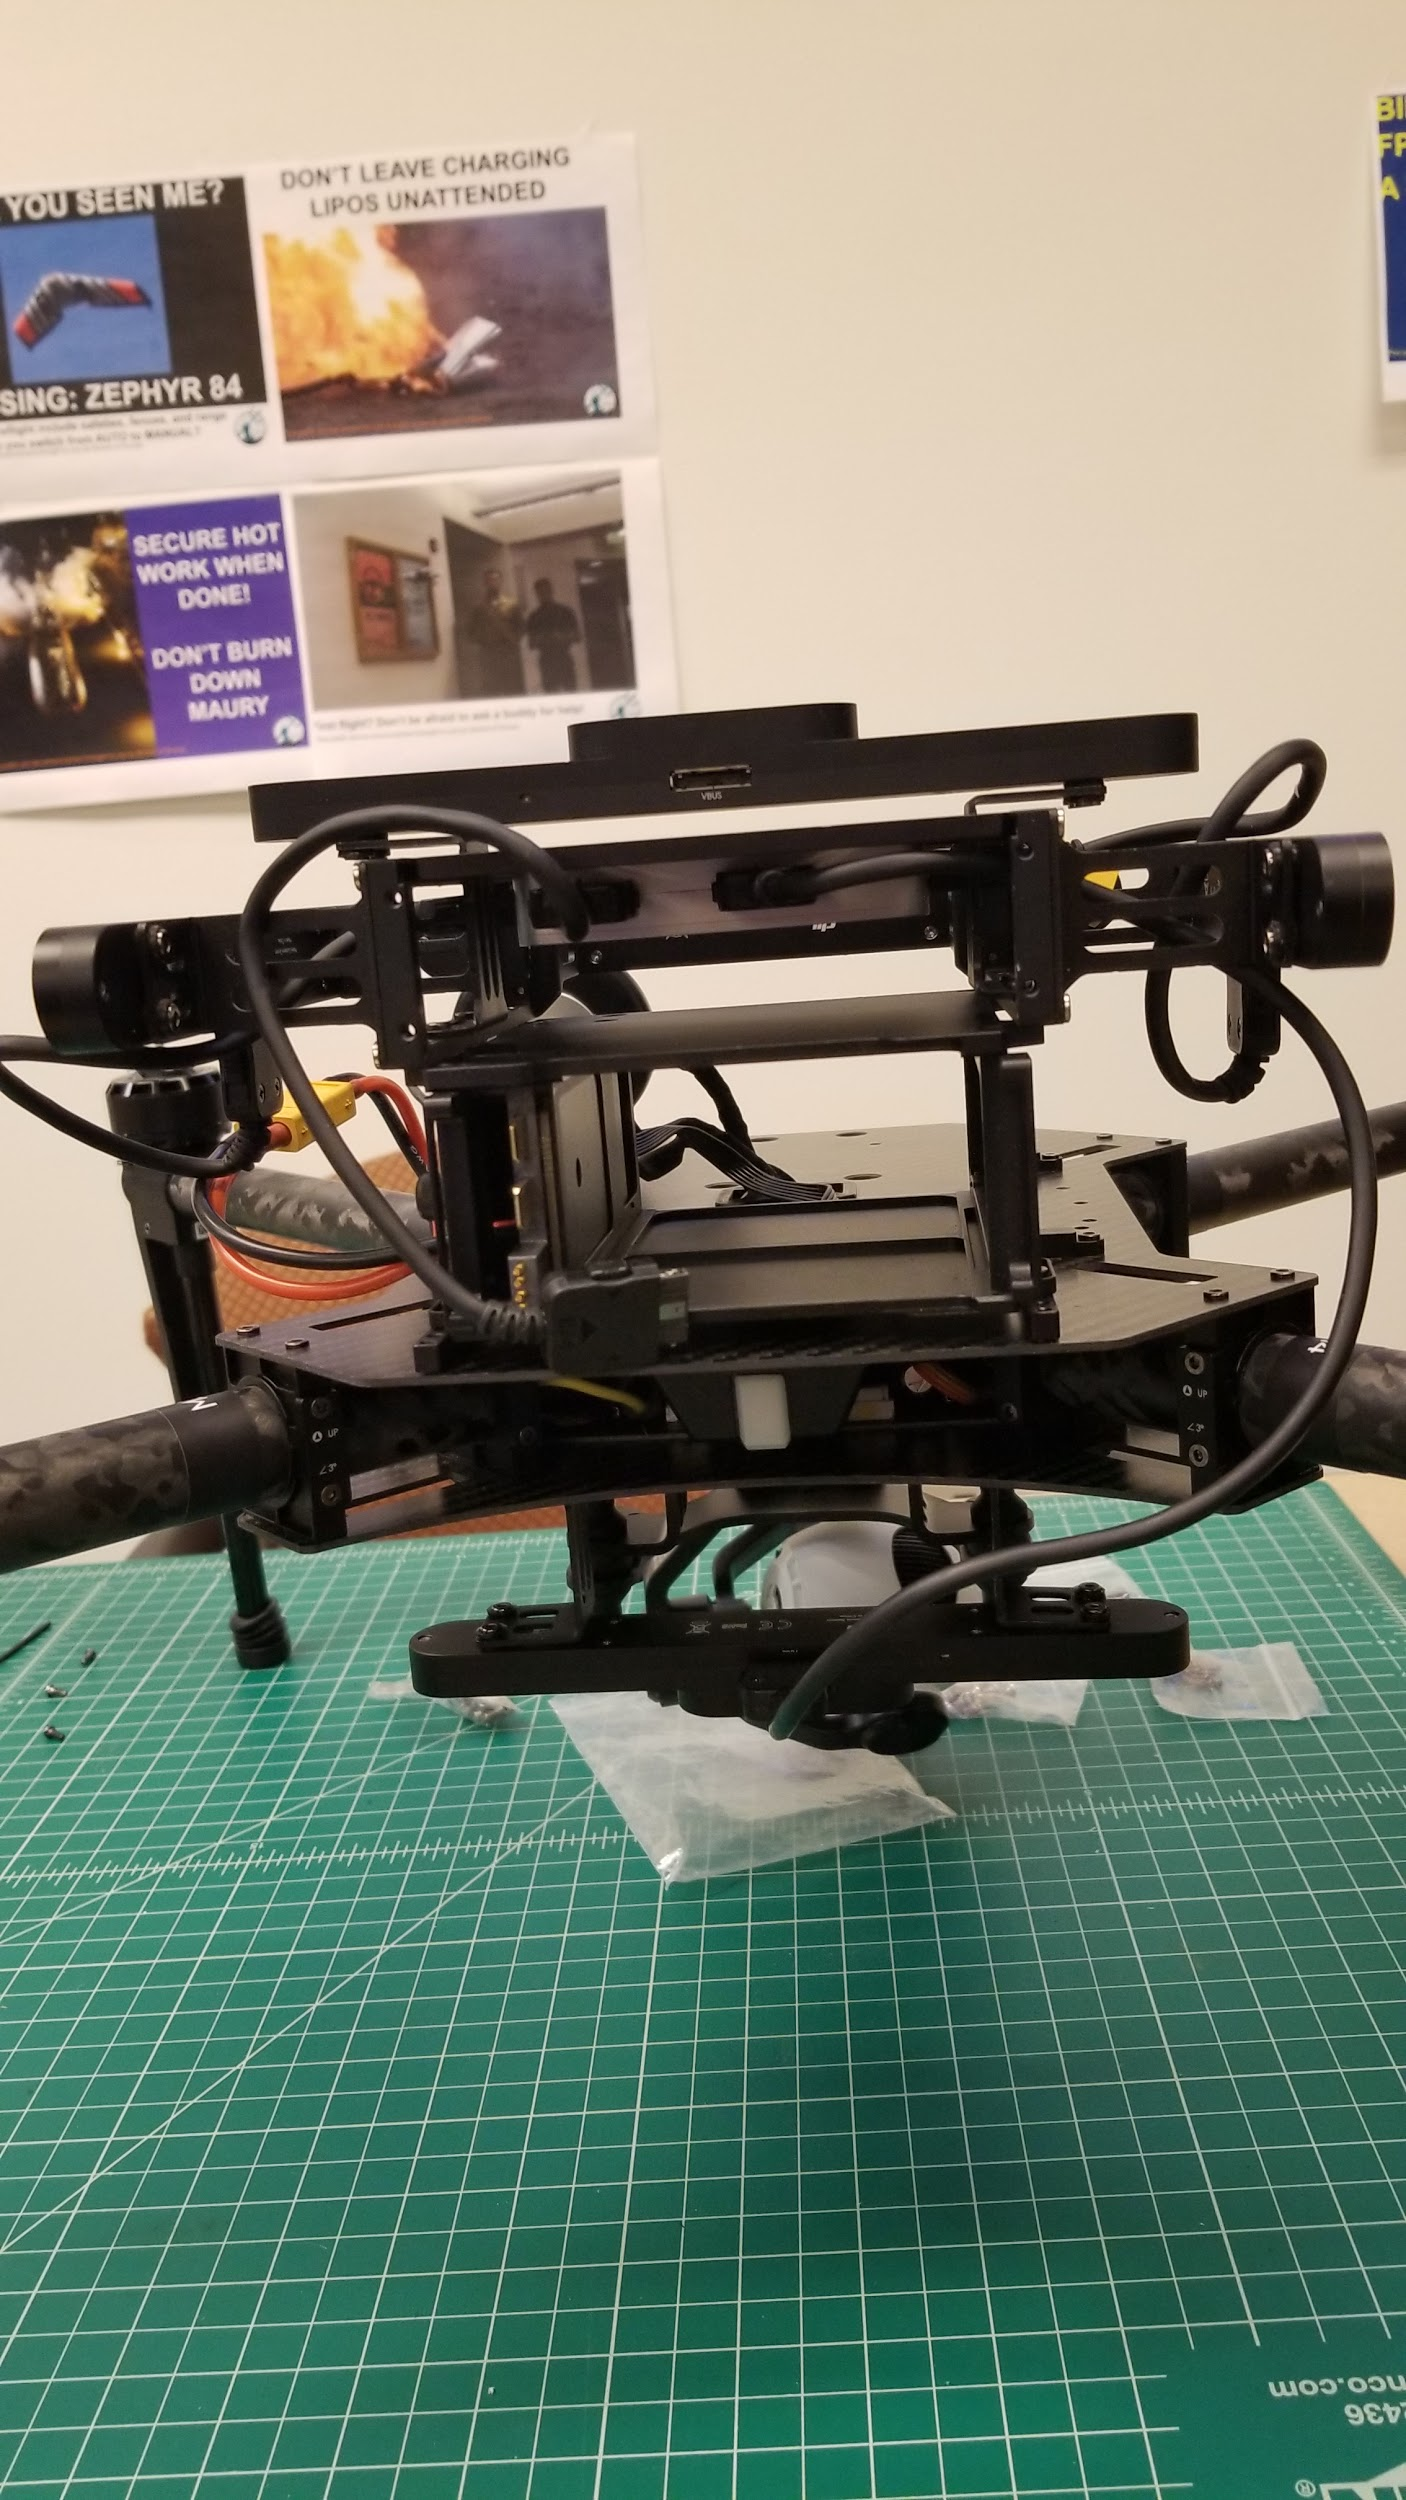
\includegraphics[width=0.8\columnwidth]{figures/hovering3.png}
\end{center}
\caption{Back view of DJI Matrice with Guidance System}
\label{fig:hovering3}
\end{figure}

\begin{figure}
\begin{center}
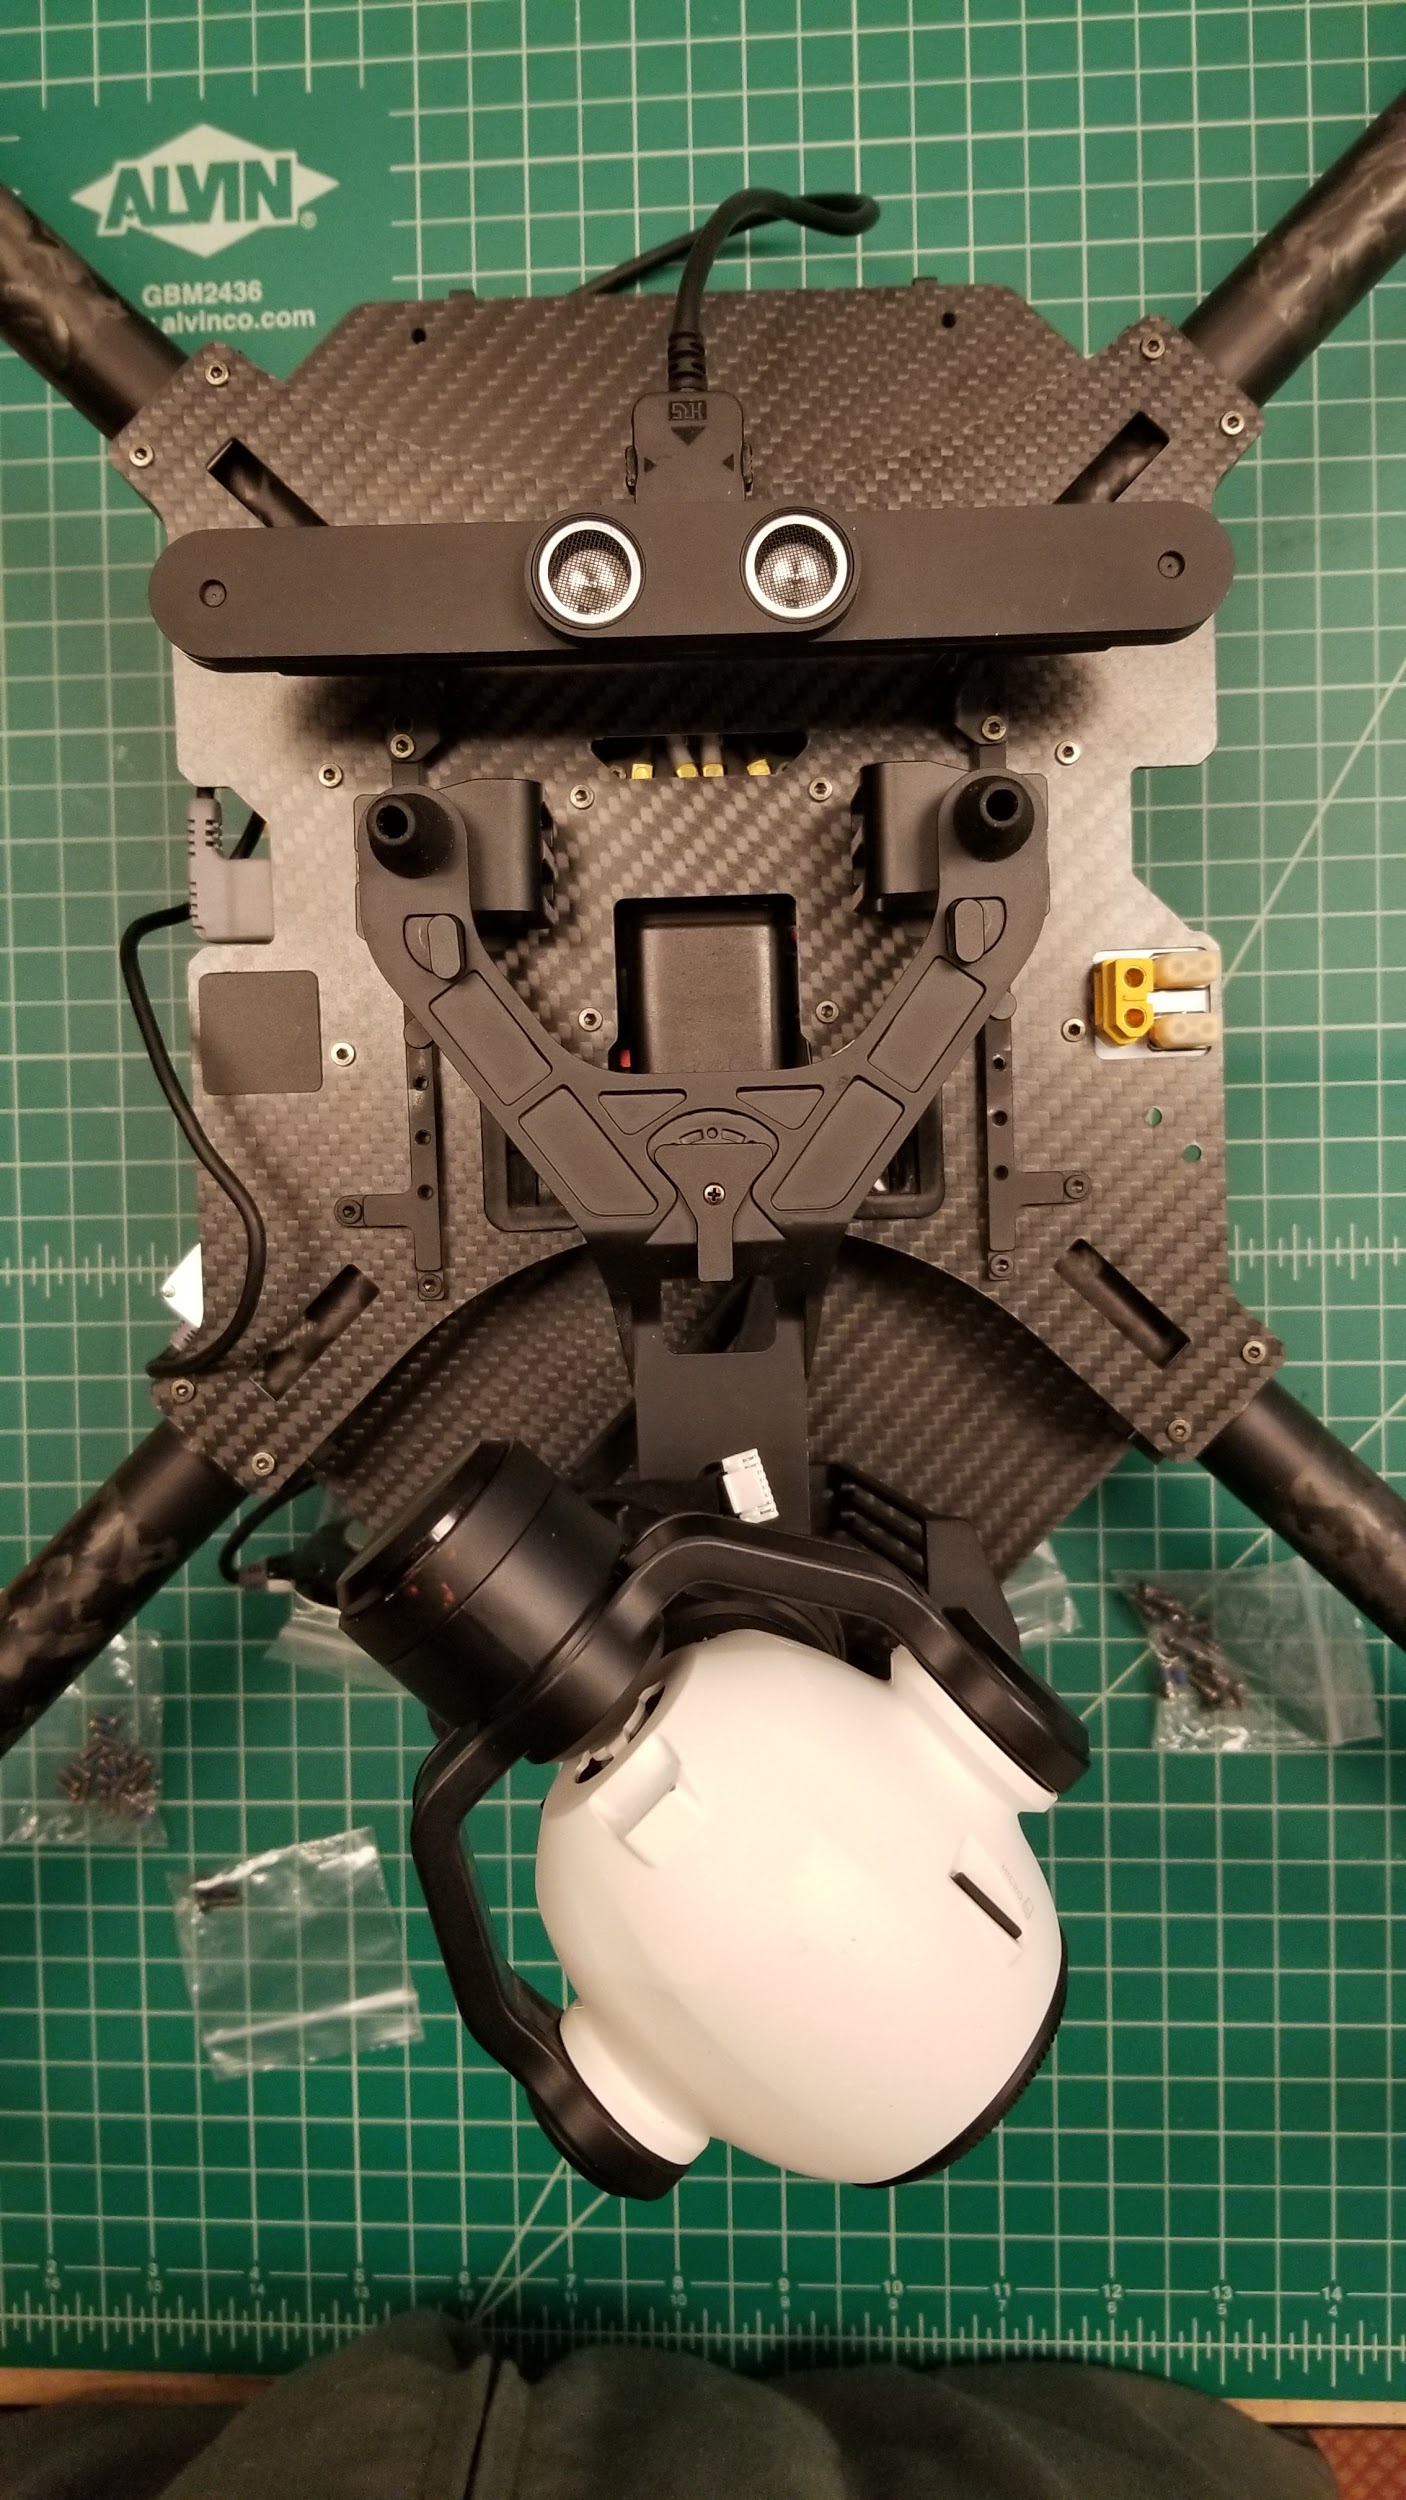
\includegraphics[width=0.8\columnwidth]{figures/hovering4.png}
\end{center}
\caption{Bottom View of Matrice 100 with bottom sensor attached}
\label{fig:hovering4}
\end{figure}

\begin{figure}
\begin{center}
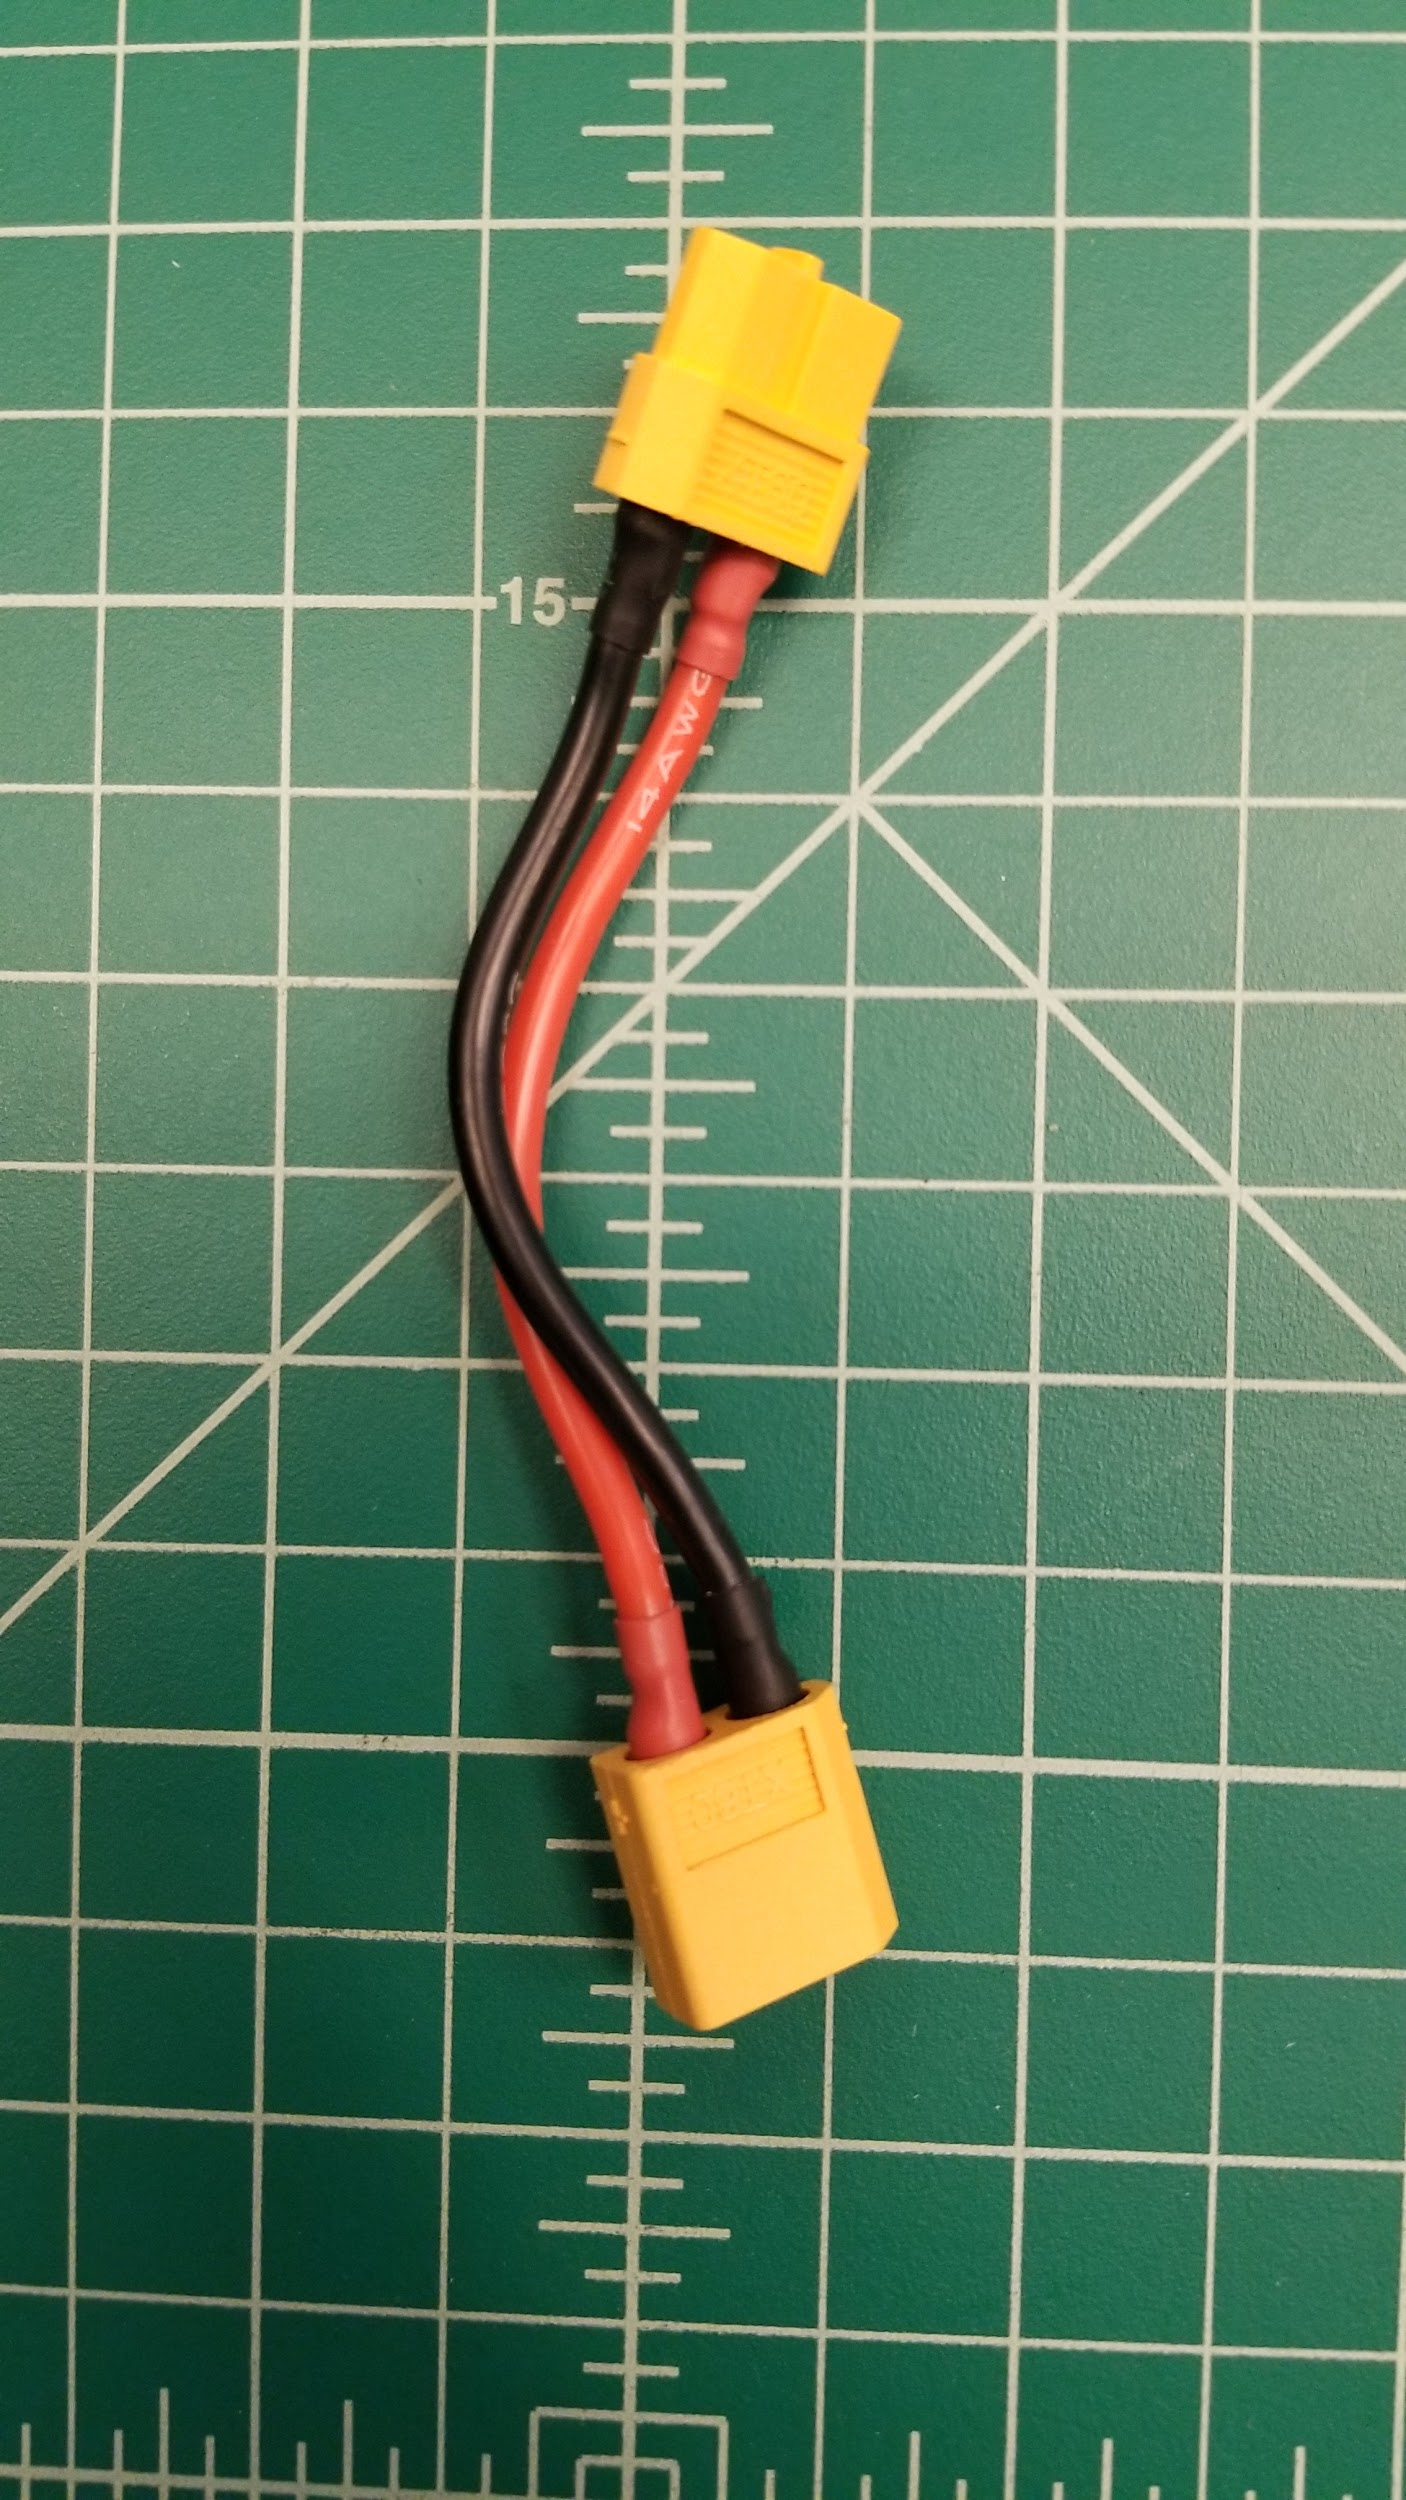
\includegraphics[width=0.8\columnwidth]{figures/hovering5.png}
\end{center}
\caption{XT60 power adapter cord needed to power guidance system. Cord length must be longer.}
\label{fig:hovering5}
\end{figure}
